\documentclass[paper=8.27in:11.69in]{scrartcl}
\usepackage{geometry}
\usepackage{graphicx}
\usepackage{pdfpages}
\usepackage{hyperref}
\usepackage{enumitem}
\usepackage{amsmath}
\DeclareMathOperator*{\argmax}{argmax}
\title{A Survey in Algorithms: Monte-Carlo Tree Search, and it's implementations in the board games.}
\author{Ulvi Bajarani, Student ID 20539914\\ \\e-mail: ulvi.bajarani01@utrgv.edu\\Class: CS 6174 Fall 2019}


\begin{document}

\maketitle

\textbf{\begin{center}
\emph{Abstract}
\end{center}
The combination of the Monte Carlo method with Tree Search revealed new possibilities to grow the programs’ strength in various board games. The first two chapters of the survey cover the basics of the Monte Carlo Tree Search (MCTS) and a brief definition of the MCTS enhancements. The most significant part of the work is dedicated to the MCTS implementations in various board games. Not explaining the rules of games, the author points out the circumstances and the results of experiments with the MCTS and its enhancements against various search algorithms, such as the default MCTS, the alpha-beta pruning, and describes the reason of some failures in some games and possible improvements of conditions. The final chapter concludes the survey, giving the relationship between the type of games and the efficiency of MCTS.}

\textbf{
\begin{center}
\emph{Keywords}
\end{center}
Monte-Carlo, Monte-Carlo Tree Search (MCTS), Selection, Expansion, Simulation, Backpropagation, alpha-beta pruning (alpha-beta search), Upper Confidence bound algorithm applied to Trees (UCT), Rapid Action Value Estimate (RAVE), Progressive Bias, Progressive Unpruning and Progressive Widening, Heavy Playouts, Decisive Moves, Monte-Carlo Solver, Go, Havannah, Hex, Lines of Actions (LOA), Amazons, Chess, Shogi.}

\section{Introduction}
Despite that Monte Carlo method, which based on random simulations, was discovered in the 1940s, only after the Ph.D. Bruce Abramson’s 1987-year thesis work “The Expected-Outcome Model of Two-Player Games” described the possibility of using the method on board games instead of static evaluation methods, which used alpha-beta search \cite{Abramson1987}. After that, it was firstly implemented in 1992 by Brügmann \cite{MaxPlanck1993MonteCG} in a board-game program for playing Go. Since then, there have been developed several realizations and improvements of the method; the most significant was combining the method with Upper Confidence bound algorithm applied to Trees (UCT), which named as Monte-Carlo Tree Search (MCTS) and described a tremendous improvement and a breakthrough in board games, such as Go, the games of Amazons, chess, Shogi etc what is a subject of the paper.\\
\subsection{Monte-Carlo Tree Search}
MCTS analyzes most prospective moves and expands the search tree, which is based on a random sampling of the extant search tree. The expansion occurs through many playouts, also called roll-outs. These playouts continue until the end; the moves of games are selected at random. The final result of the games is used to update the weight of game tree nodes: the better the result of the node is, the higher the probability that the move is chosen in future playouts. In Pure Monte Carlo Game Search, the number of initial playouts is limited to a number. However, the efficiency of search rises with time, as more playouts are assigned to the moves with a high winning frequency according to the results of previous playouts. Monte-Carlo Tree Search consists of four sequential stages:

\begin{enumerate}[label=\arabic*)]
\item Selection – Starting from a root R, which is a game state, the most successive nodes are traversed till leaf L, which is the move that has not been simulated.
\item Expansion – Until a leaf L ends with a possible result, child nodes of C are created. Then, one of the child nodes is chosen until a possible result is found.
\item Simulation – a random playout of child node C.
\item Backpropagation – propagate the results through the tree from C to L and R and update their information.
\item Final Decision – After several iterations of steps from 1 to 4, the final move is selected.
\end{enumerate}


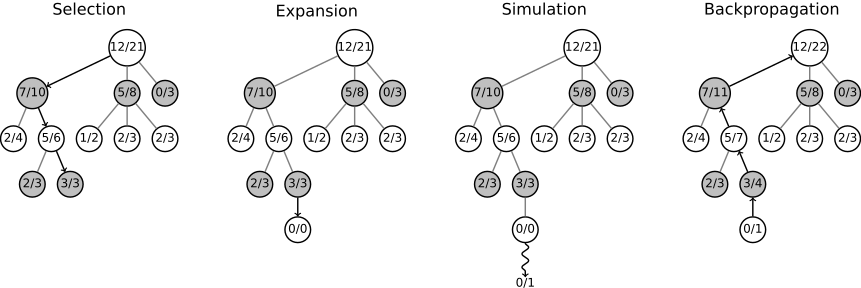
\includegraphics[scale=0.6]{MCTS}

\subsection{Markov Decision Processes}
How might a powerful method such as the Monte-Carlo Tree Search be modeled? The decision problems are frequently modeled in Markov Decision Processes, which is a composition of 

\begin{itemize}

\item States $ s \in S $, where s is a general state of the system, and $ S_{t} \in S $  is a particular state of the system at time $ t $.
\item Actions $ a \in A $, where a is a general action of the system and $ A_{t} \in A (S_{t}) $  is a particular action of the system at time $ t $, which is chosen from available actions in   $ S_{t} $. In the case where there are no moves in $ a $ state, then the state is called terminal, which is possible in endgame positions.
\item Transition probabilities $ p (s^{'} | s, a) $ is the probability of moving to state $ s^{'} $ by choosing state $ s $ from action $ a $.
\item Rewards $ p (s, a, s^{'}) $ is the value of expected reward after choosing action $ a $ in state $ s $ and moving to the new state $ R_{t+1} $, which is equal to $r( S_{t}, A_{t}, S_{t+1} $).
\item The reward discount rate $ \gamma  \in [0; 1] $ is the parameter that reduces the importance of later-received rewards.

\end{itemize}

To make a choice between actions, the policy $\pi(a \ | \ s)$ is used, which defines the probability of selecting action a in the state s. In order to solve the MDP tasks, which might be either episodic or continuous, the value of return $ S_{t} $ , which is also called a cumulative discounted reward, should be maximized by either
\\
\\
$ G_{t} = \sum_{k = 0}^{\infty} \gamma^{k}{R}_{t+k+1} = {R}_{t+1} + \gamma{R}_{t+2} + \gamma^{2}{R}_{t+3} \ \ldots $
\\
\\
or
\\
\\
$ G_{t} = \sum_{k = 0}^{T-t-1} \gamma^{k}{R}_{t+k+1} = {R}_{t+1} + \gamma{R}_{t+2} + \gamma^{2}{R}_{t+3} \ \ldots \gamma^{k}{R}_{T} $\\

for episodic tasks, where $ T-t $ is the remaining duration of the episode.
\subsection{Upper Confidence bound algorithm applied to Trees (UCT)}
Another problem is the behavior of MCTS: Should the tree-search decide whether the move is worth analyzing deeply (exploitation) or find other possible alternatives and analyze them (an exploration)? The problem is similar to the multi-armed bandit problem, which also requires a decision with limited resources. There are several possible solutions to optimize such processes in MCTS, but the most frequently used approach is the Upper Confidence bound algorithm applied to Trees (UCT). There is a possible formula of UCT, which maximizes the score of $ {s}_{1} $:

\begin{equation}
\label{eq:Formula1}
z = {s}_{1} \leftarrow \ \argmax_{j \in C_{s_{1}}} [\frac{{w}_{j}}{{n}_{j}} + K \ \sqrt{\frac{\ln({C_{s_{1}})}}{n_{j_{1}}}}]
\end{equation}

Where 
$ {s}_{1} $ is the score of $ {s}_{1} $, $ {C_{s_{1}}} $ is the child nodes of $ {s_{1}} $, $ {w_{j}} $ is the number of wins for the j node, $ {n_{j}} $ is the number of playouts for the node $ j $, $ {n_{s_{1}}} $ is the number of playouts for node $ {s_{1}} $, and $ K $ is an exploration parameter to keep the balance between exploitation and exploration.\\

It should be noticed that the efficiency of choice depends on not only the number of simulations, but also the time consumed on stages: when there are many games in a node, it is accurate to spend much more time on the selection, however, the simulation strategy gives a higher accuracy when the number of games in node is few. \cite{Kocsis06banditbased}\\
\section{Enhancements of MCTS}
There are several enhancements to MCTS. In section 2, the main ones are described.\\
\subsection{Rapid Action Value Estimate (RAVE)}
Suppose that we have $ {m}_{i} $ moves leading from $ s $ to $ {s}_{i}^{'} $. In the MCTS algorithm, only the number of playouts $ {n}_{s} $ and winning playouts $ {w}_{s} $ are stored. While in RAVE, the number and winning playouts from $ s $ to $ {s}_{i}^{'} $ are stored not only in $ s $ but also in  $ {m}_{i} $ moves as $ {n}^{'}_{s, s^{'}_i} $ and $ {w}^{'}_{s, s^{'}_i} $, respectively. This might significantly increase the bias of selection by adding a RAVE Score in the formula \ref{eq:Formula1}:

\begin{equation}
\label{eq:Formula2}
z = {s}_{1} \leftarrow \ \argmax_{j \in C_{s_{1}}} [(1 - \beta ) \ \frac{{w}_{j}}{{n}_{j}} + \beta \ {\frac{{w^{'}_{s_{1,j}}}}{n^{'}_{s_{1,j}}}} + \ K \ \sqrt{\frac{\ln({C_{s_{1}})}}{n_{j_{1}}}}
\end{equation}

,
where \beta \ is a parameter approaching to 0 when $ {n}_{j} $ tends to infinity.\\

The possible enhancements and diversities of RAVE are:\\
\begin{itemize}

\item PoolRave biasing moves in the simulation step;
\item The Last-Good-Reply (LGR), which stores the last best reply to a previous move and tests it in the playouts of other moves;
\item Move-Average Sampling Technique (MAST) which is similar to PoolRave but stores the evaluation of all moves globally;
\item N-gram Average Sampling Technique, which is similar to LGR, but stores the move with the highest winning percentage;
\end{itemize}
\subsection{Progressive Bias}
The approach here is similar to RAVE, however, instead of using the statistics of MCTS simulation, a heuristic function with progressively decaying influence is used:
\[z = {s}_{1} \leftarrow \ \argmax_{j \in C_{s_{1}}} [(1 - \beta ) \ \frac{{w}_{j}}{{n}_{j}} + \beta \ {\frac{{w^{'}_{s_{1,j}}}}{n^{'}_{s_{1,j}}}} + \ K \ \sqrt{\frac{\ln({C_{s_{1}})}}{n_{j_{1}}}} + f({n_{j_{1}}})\],
where $ f({n_{j_{1}}}) $ is a function with an heuristic evaluation of child node, which might be described as $ \frac{k_{bias}  \ * \ H(n_{i})}{n_{i}} $, where $ {k_{bias}} $ is a suitable constant for an heuristic function, and $ H(n_{i}) $ is an heuristic function.\\
\subsection{Progressive Unpruning and Progressive Widening}
Progressive Unpruning \cite{Chaslot2008ProgressiveSF} and Progressive Widening \cite{Coulom2007ComputingR} are similar approaches to optimize an expansion stage. After the first evaluation of nodes during exploration, nodes with poor heuristic scores are going to be pruned till the time when the node is better exploited; then, the nodes are going to be “unpruned.” The only difference is in the realizations: While Progressive Unpruning doesn’t explore a small number of child nodes, Progressive Widening prunes child nodes only after some number of simulations.\\
\subsection{Decisive Moves}
Another possible enhancement is spending more time to analyze moves, which might lead to a decisive result. If it is proved that the move leads to a decisive result, it is going to be played without any consideration of other moves’ evaluations, which performed better results against random searches, even though it may have taken more time \cite{Teytaud2010OnTH}. Moreover, the moves preventing decisive moves might also be implemented, which is the subject of further improvements.\\
\subsection{Heavy Playouts}
The simulation strategy, where the number and speed of simulations are decreased to improve their accuracy. In this case, domain knowledge are used, which might be either implemented patterns \cite{Wang2007ModificationsOU}, or some heuristic function \cite{Winands2009EvaluationFB}.\\
\subsection{Monte-Carlo Solver}
Another approach similar to Decisive Moves is the Monte-Carlo Solver. The solver proves the game-theoretical value of a node when it is possible. Monte-Carlo Solver proves only game-theoretical value wins or losses, because, in a terminal-game state, the value is already proven. When at least one of the child nodes is proven to lose, or proven losing, the node is proven winning; when at all children nodes are proven winning, the node is proven losing \cite{WinandsBS08}. In such a case, the proven node gets the reward either as $-\infty$ or $+\infty$, a lose and win, respectively. Then, a node with a proven node tries to deduce the evaluation.\\
\section{The experimental results in games}
\subsection{Go}
Since Brügmann \cite{MaxPlanck1993MonteCG} described the possibility of usage Monte-Carlo Search for the game Go with his program Gobble, there were several experiments conducted, the first of which was conducted on a 9x9 board. Despite the fact that that the implementation of eyes was slightly different than in Gobble, and adding Progressive Pruning improved the random games generation speed, it was not sufficient to outperform GNU Go, which was based on an alpha-beta search and domain-dependent knowledge \cite{Bouzy2003MonteCarloGD}; in parallel, the tests showed that adding domain-knowledge such as $3x3$ patterns increased the performance of Monte-Carlo Search when compared with a random Monte-Carlo Search, likewise a move-generator using Progressive Pruning \cite{Bouzy2005AssociatingDK}. Moreover, comparing to a random Monte-Carlo Search, the domain-knowledge did search in the boards with more intersections (13x13 and 19x19) more effective.

The major breakthrough was in 2007, when Rémi Coulom, unlike his predecessors, first combined Tree Search with the Monte-Carlo method in his Crazy Stone program, which was also successfully used in other games \cite{Coulom2006EfficientSA}. The approach was calculating the value of all nodes (unlike Monte-Carlo Search, which passed only the evaluation of the end of nodes) by the formula below and pass them through root:\\

\begin{equation}
\label{eq:Formula3}
u_{i} = \textup{exp}(-2.4\frac{{{\mu}_{0}} - {{\mu}_{i}}}{\sqrt{2(\sigma_{0}^{2} + \sigma_{i}^{2}})}) + \epsilon_{i}
\end{equation}

where $u_{i}$ is the urgency of move $i$, ${\mu}_{i}$ is the estimated value of move $i$ (${{\mu}_{0}} > {{\mu}_{i}}$), $\sigma_{i}^{2}$ is a variance of move $i$, and $\epsilon_{i}$ is a constant which equals to \\

\begin{equation}
\label{eq:Formula4}
\epsilon_{i} = \frac{0.1 + 2^{-i} + a_{i}}{N}
\end{equation}

and prevents the urgency of a move becoming equal to zero. In the formula, $N$ equals to the total number of analyzed moves, and $a_{i}$ equals to 1 in atari and 0 in otherwise.\\
Another successful test was with the MoGo program, which, unlike Crazy Stone, was based on the UCT program \cite{Gelly2011MonteCarloTS}. In the first experiment of this program, the RAVE search combined with MCTS and UCT outperformed against GNUGo with a winning percentage above 52\%; in the second approach, adding heuristic functions outplayed GNUGo with a winning percentage from 69\% up to 97\%. As a result of the researches, nowadays, all top Go Programs are based on the MCTS search.
\subsection{Lines of Actions}
For the game of Lines of Actions, MC-LOA program used MCTS with UCT, Progressive Bias and mixed strategy, containing several strategies such as:

\begin{itemize}
\item Evaluation Cut-Off to terminate the simulated game with high percentage.\\
\item Corrective Strategy to minimize the risk of dubious moves;\\
\item Greedy Strategy to reduce the number of analyzed moves.\\
\end{itemize}

It should be noticed that, instead of dividing to the number of games, Progressive Bias used $f({l_{j_{1}}})$ function dividing number of losses in the node ${j_{1}}$:\\

$f({l_{j_{1}}}) = \frac{k_{bias}  \ * \ P_{mc}}{l_{j_{1}}+ 1}$\\

where $k_{bias}$ is a constant, $P_{mc}$ $l_{j_{1}}$ is the transition probability of a move category mc, and 1 is a dominator to avoid the division to 0.\\

Experiments with MIA III, MIA 4.5, and the default version of MC-LOA described threshold value of evaluation cut-off equal to 700 as the best. An MC-LOA with mixed strategy performed better against other strategies. While MC-LOA with mixed strategy solved more endgame positions than non-variable-depth alpha-beta search, it could not outperform classic alpha-beta search of MIA 4.5. In direct matches against single-thread MIA 4.5, single-threaded MC-LOA scored almost with 47 ±3.1\%. However, increasing the number of threads even up to 2 in MC-LOA rose the winning percentage of single-thread MIA 4.5 to 56\%, because the efficiency of MC-LOA’s search increased during parallelization. Moreover, recycling significant part of tree and using $\sqrt{{l_{j_{1}}+ 1}}$ instead of ${l_{j_{1}}}$ rose the winning percentage of single-threaded MC-LOA with mixed strategy to 52\%, making Progressive Bias more relevant\cite{Winands2010MonteCT}.
\subsection{Hex}
The MoHex program, which used MCTS with some enhancements, such as a parallel solver based on depth-first proof number (DFPN) search, experienced high success, winning the Computer Olympiad in 2009. In the experimental tournaments, it scored more than 70\% against program Six and equal results against another program, Wolve. Both opponents used the alpha-beta approach to find the best move \cite{Arneson2010MonteCT}. Another experimental research that used the Rapid Action Value Estimation (RAVE) algorithm described an inverse proportionality between a winning percentage and the value of UCT constant when the RAVE algorithm is used \cite{Cazenave2010MonteCarloH}.
\subsection{Havannah}
There were conducted several kinds of research independent of each other:\\

\begin{enumerate}[label=\arabic*)]
\item The results of research by Stankiewicz, Winands, and Uiterwijk \cite{Stankiewicz2011MonteCarloTS} and their simulations against default MCTS for Havannah showed that:\\

\begin{itemize}

\item The Last-Good-Reply (LGR) generally improves the performance of MCTS. The best results occurred in the strategy called Last-Good-Reply with forgetting-1 (LGRF-1) when LGR did not test the move that leads to a loss in the playouts. (up to 62\% winning percentage).
\item N-gram Average Sampling Technique also improves the performance of the MCTS search (up to 61\% winning percentage). Moreover, the combination of LGR and N-gram together improved the performance better than separately, but the growth was slight when compared (up to 66\% winning percentage).
\item Enhancing the selection step in MCTS by initialing the win counts and visit counts of new nodes with the values based on the results of corresponding moves, and biasing the search to certain types of moves, such as identifying joint and neighbour moves or local connections or edge and corner connections raises the performance of MCTS search (up to 69\% winning percentage); Combination of these methods increased the winning up to 73\% winning percentage.
\item However, the most dramatic increase was when both the enhancement combined by the combination of LGRF-2 (similar to LGRF-1, but with forgetting two previous moves) and N-gram strategy with decay value \gamma equal to 0 and \epsilon-greedy policy equal to 0.1 (up to 77.6\% winning percentage). However, the results also described that using only identifying joint and neighbor moves as enhancement might be enough in the combination of methods.
\end{itemize}
\item Joris Duguépéroux, Ahmad Mazyad, Fabien Teytaud, Julien Dehos \cite{Duguproux2016PruningPI} and their simulations against default MCTS for Havannah showed that:

\begin{itemize}

\item The performance of MCTS and RAVE might be increased by choosing the proper value of constant K in formulas \ref{eq:Formula1} and \ref{eq:Formula3} described above. Additionally, RAVE search described better results against classical MCTS.\\
\item Progressive History, which is a combination of both Progressive Bias and History Heuristic, performed better than RAVE and scored up to 73\% against standard MCTS algorithm.
\item Extended RAVE, which is a combination of both RAVE and Progressive History, was hardly slower than RAVE and outperformed RAVE with a winning rate.
\item RAVE with Havannah-Mate strategy, which finds immediate wins in 4 half-moves during playouts, required much more time than MCTS with random playouts and didn’t give any significant advantages in long games. Implementing such fact and using Havannah-Mate for the first-third of playouts gave almost 60\% against RAVE with random playouts.
\item The most significant improvement was when Progressive History used with Havannah-Mate; such a strategy scored almost 70\% against classical MCTS. Another attractive approach by the same authors \cite{Duguproux2016PruningPI} used Progressive Widening, which was described in the article “Playout Pruning with Rave” (PPR). Experiments described the superiority of PPR against other playout improvements, such as RAVE, PoolRAVE, MAST, NAST, and LGRF1; the superiority increased proportionality to the size of the board.
\end{itemize}

\end{enumerate}
\subsection{Amazons}
Using only UCT search increased Vanilla’s win rate up to 81.6\% against standard MCTS algorithm, while without UCT, the best result of the combination of average score and Win-Loss ratio was only 63.5\%. However, the results dramatically increase with an accessibility evaluation for Amazons, which is a probability of accessing a square \cite{Kloetzer2007TheMA}.\\
\subsection{Chess}
Despite the fact that the combination of algorithms, such as decisive moves, progressive bias, Heavy Playouts with \epsilon-greedy policy equal to 0.4 and Static Exchange Evaluator, which examines all captures in a square, and endgame tablebases increased the strength of MCTS program for chess up to 864 Elo points compared to standard MCTS algorithm; the significant part of improvement was made by Heavy Playouts and Decisive moves. However, it was proven that even with such improvements, MCTS is not suitable to apply in chess and compete against the standard alpha-beta algorithm \cite{Arenz}. The main reason for this is the speed of the search algorithm, which could not identify search traps. Another problem described by standard MCTS algorithm was that the results of simulations were based on positional values, rather than the material of sides. Furthermore, standard MCTS had a difficulty to end a decisive advantage with a mate in simulations and ends them draw; this is solved by decreasing value simulations ended drawn. Despite such results, after the success of the AlphaGo program \cite{Silver2017MasteringCA}, which used MCTS for reinforcement Learning, MCTS is used by some robust programs as an enhancement of alpha-beta algorithm, which is a subject of future improvements. According to Mark Lefler, who is the one of authors Komodo 13.2.5, the idea is using short alpha-beta search in the child nodes of tree search and updating the values of nodes and root \cite{SiteInterview}. \\
\subsection{Shogi}
MCTS search engine, using various methods such as assigning an Elo rating to moves, human games and an open book to define the weight of moves, progressive widening, killer moves, and history heuristics, was able to win only 4\% percent of games against TOHMI program, which didn’t use MCTS methods and was based on a search and evaluation function \cite{Sato2010ASP}. There were two possible reasons for this failure:\\

\begin{enumerate}[label=\arabic*)]

\item The evaluation of minor tactical losses, which put the program in a long-term disadvantage;
\item When MCTS was in situations with a disadvantage, it made move decisions that counted as inferior in TOHMI. The quiescence search reducing win rate was used to deal with this problem: when the quiescence search was used, the win rate rose to 32\%.

\end{enumerate}

Despite the results against TOHMI in games, and the results of tactical tests, which wasn’t as high TOHMI, the MCTS search increased the quality of opening moves, and showed an endgame evaluation which most Shogi programs couldn’t be enabled to reach \cite{Sato2010ASP}.\\
\section{Conclusion}
MCTS, with its enhancements, is a robust search algorithm, which might sufficiently compete against an alpha-beta search in board games. However, while MCTS outperforms alpha-beta in strategical games as Hex, Lines of Actions, and Amazons due to the number of simulations, implementing MCTS in the tactical games with the highest number of search traps, such as Shogi and Go does not outperform the classic alpha-beta search. In addition to different enhancements of MCTS, in some games, such as Havannah and Go, the heuristic knowledge is required.

\bibliographystyle{unsrt}
\bibliography{references6174}

\end{document}